% $Header: /u/gcmpack/manual/s_autodiff/text/doc_ad_2.tex,v 1.4 2001/10/05 22:22:20 heimbach Exp $
% $Name:  $

{\sf Automatic differentiation} (AD), also referred to as algorithmic
(or, more loosely, computational) differentiation, involves 
automatically deriving code to calculate
partial derivatives from an existing fully non-linear prognostic code.
(see \cite{gri:00}).
A software tool is used that parses and transforms source files 
according to a set of linguistic and mathematical rules. 
AD tools are like source-to-source translators in that
they parse a program code as input and produce a new program code 
as output.
However, unlike a pure source-to-source translation, the output program
represents a new algorithm, such as the evaluation of the
Jacobian, the Hessian, or higher derivative operators.
In principle, a variety of derived algorithms
can be generated automatically in this way.

The MITGCM has been adapted for use with the
Tangent linear and Adjoint Model Compiler (TAMC) and its successor TAF
(Transformation of Algorithms in Fortran), developed
by Ralf Giering (\cite{gie-kam:98}, \cite{gie:99,gie:00}).
The first application of the adjoint of the MITGCM for senistivity
studies has been published by \cite{maro-eta:99}.
\cite{sta-eta:97,sta-eta:01} use the MITGCM and its adjoint
for ocean state estimation studies.
In the following we shall refer to TAMC and TAF synonymously,
except were explicitly stated otherwise.

TAMC exploits the chain rule for computing the first
derivative of a function with
respect to a set of input variables. 
Treating a given forward code as a composition of operations --
each line representing a compositional element, the chain rule is
rigorously applied to the code, line by line. The resulting 
tangent linear or adjoint code,
then, may be thought of as the composition in 
forward or reverse order, respectively, of the
Jacobian matrices of the forward code's compositional elements.

%**********************************************************************
\section{Some basic algebra}
\label{sec_ad_algebra}
%**********************************************************************

Let $ \cal{M} $ be a general nonlinear, model, i.e. a
mapping from the $m$-dimensional space 
$U \subset I\!\!R^m$ of input variables 
$\vec{u}=(u_1,\ldots,u_m)$
(model parameters, initial conditions, boundary conditions
such as forcing functions) to the $n$-dimensional space 
$V \subset I\!\!R^n$ of 
model output variable $\vec{v}=(v_1,\ldots,v_n)$ 
(model state, model diagnostcs, objective function, ...) 
under consideration,
%
\begin{equation}
\begin{split}
{\cal M} \, : & \, U \,\, \longrightarrow \, V \\
~      & \, \vec{u} \,\, \longmapsto \, \vec{v} \, = \, 
{\cal M}(\vec{u}) 
\label{fulloperator}
\end{split}
\end{equation}
%
The vectors $ \vec{u} \in U $ and $ v \in V $ may be represented w.r.t.
some given basis vectors
$ {\rm span} (U) = \{ {\vec{e}_i} \}_{i = 1, \ldots , m} $ and
$ {\rm span} (V) = \{ {\vec{f}_j} \}_{j = 1, \ldots , n} $ as
\[
\vec{u} \, = \, \sum_{i=1}^{m} u_i \, {\vec{e}_i},
\qquad
\vec{v} \, = \, \sum_{j=1}^{n} v_j \, {\vec{f}_j}
\]

Two routes may be followed to determine the sensitivity of the 
output variable $\vec{v}$ to its input $\vec{u}$.

\subsection{Forward or direct sensitivity}
%
Consider a perturbation to the input variables $\delta \vec{u}$
(typically a single component 
$\delta \vec{u} = \delta u_{i} \, {\vec{e}_{i}}$).
Their effect on the output may be obtained via the linear
approximation of the model $ {\cal M}$ in terms of its Jacobian matrix
$ M $, evaluated in the point $u^{(0)}$ according to
%
\begin{equation}
\delta \vec{v} \, = \, M |_{\vec{u}^{(0)}} \, \delta \vec{u}
\label{tangent_linear}
\end{equation}
with resulting output perturbation $\delta \vec{v}$.
In components
$M_{j i} \, = \, \partial {\cal M}_{j} / \partial u_{i} $, 
it reads
%
\begin{equation}
\delta v_{j} \, = \, \sum_{i} 
\left. \frac{\partial {\cal M}_{j}}{\partial u_{i}} \right|_{u^{(0)}} \, 
\delta u_{i}
\label{jacobi_matrix}
\end{equation}
%
Eq. (\ref{tangent_linear}) is the {\sf tangent linear model (TLM)}.
In contrast to the full nonlinear model $ {\cal M} $, the operator
$ M $ is just a matrix
which can readily be used to find the forward sensitivity of $\vec{v}$ to 
perturbations in  $u$,
but if there are very many input variables $(\gg O(10^{6})$ for 
large-scale oceanographic application), it quickly becomes 
prohibitive to proceed directly as in (\ref{tangent_linear}),
if the impact of each component $ {\bf e_{i}} $ is to be assessed. 

\subsection{Reverse or adjoint sensitivity}
%
Let us consider the special case of a
scalar objective function ${\cal J}(\vec{v})$ of the model output (e.g. 
the total meridional heat transport, 
the total uptake of $CO_{2}$ in the Southern 
Ocean over a time interval,
or a measure of some model-to-data misfit)
%
\begin{eqnarray}
\begin{array}{cccccc}
{\cal J}  \, : &  U & 
\longrightarrow & V &   
\longrightarrow & I \!\! R \\
~       &  \vec{u} & \longmapsto     & \vec{v}={\cal M}(\vec{u}) & 
\longmapsto     & {\cal J}(\vec{u}) = {\cal J}({\cal M}(\vec{u}))
\end{array}
\label{compo}
\end{eqnarray}
%
The perturbation of $ {\cal J} $ around a fixed point $ {\cal J}_0 $,
\[
{\cal J} \, = \, {\cal J}_0 \, + \, \delta {\cal J}
\]
can be expressed in both bases of $ \vec{u} $ and $ \vec{v} $
w.r.t. their corresponding inner product 
$\left\langle \,\, , \,\, \right\rangle $ 
%
\begin{equation}
\begin{split}
{\cal J} & = \,
{\cal J} |_{\vec{u}^{(0)}} \, + \, 
\left\langle \, \nabla _{u}{\cal J}^T |_{\vec{u}^{(0)}} \, , \, \delta \vec{u} \, \right\rangle 
\, + \, O(\delta \vec{u}^2) \\
~ & = \,
{\cal J} |_{\vec{v}^{(0)}} \, + \, 
\left\langle \, \nabla _{v}{\cal J}^T |_{\vec{v}^{(0)}} \, , \, \delta \vec{v} \, \right\rangle
\, + \, O(\delta \vec{v}^2)
\end{split}
\label{deljidentity}
\end{equation}
%
(note, that the gradient $ \nabla f $ is a co-vector, therefore
its transpose is required in the above inner product).
Then, using the representation of 
$ \delta {\cal J} = 
\left\langle \, \nabla _{v}{\cal J}^T \, , \, \delta \vec{v} \, \right\rangle $,
the definition 
of an adjoint operator $ A^{\ast} $ of a given operator $ A $,
\[ 
\left\langle \, A^{\ast} \vec{x} \, , \, \vec{y} \, \right\rangle =
\left\langle \, \vec{x} \, , \,  A \vec{y} \, \right\rangle 
\]
which for finite-dimensional vector spaces is just the 
transpose of $ A $,
\[
A^{\ast} \, = \, A^T
\]
and from eq. (\ref{tangent_linear}), (\ref{deljidentity}),
we note that
(omitting $|$'s):
%
\begin{equation}
\delta {\cal J}
\, = \,
\left\langle \, \nabla _{v}{\cal J}^T \, , \, \delta \vec{v} \, \right\rangle
\, = \,
\left\langle \, \nabla _{v}{\cal J}^T \, , \, M \, \delta \vec{u} \, \right\rangle
\, = \, 
\left\langle \, M^T \, \nabla _{v}{\cal J}^T \, , \, 
\delta \vec{u} \, \right\rangle
\label{inner}
\end{equation}
%
With the identity (\ref{deljidentity}), we then find that
the gradient $ \nabla _{u}{\cal J} $ can be readily inferred by 
invoking the adjoint $ M^{\ast } $ of the tangent linear model $ M $
%
\begin{equation}
\begin{split}
\nabla _{u}{\cal J}^T |_{\vec{u}} & 
= \, M^T |_{\vec{u}} \cdot \nabla _{v}{\cal J}^T |_{\vec{v}}  \\
~ & = \, M^T |_{\vec{u}} \cdot \delta \vec{v}^{\ast} \\
~ & = \, \delta \vec{u}^{\ast}
\end{split}
\label{adjoint}
\end{equation}
%
Eq. (\ref{adjoint}) is the {\sf adjoint model (ADM)}, 
in which $M^T$ is the adjoint (here, the transpose) of the 
tangent linear operator $M$, $ \delta \vec{v}^{\ast} $ 
the adjoint variable of the model state $ \vec{v} $, and
$ \delta \vec{u}^{\ast} $ the adjoint variable of the control variable $ \vec{u} $.

The {\sf reverse} nature of the adjoint calculation can be readily 
seen as follows. 
Consider a model integration which consists of $ \Lambda $
consecutive operations
$ {\cal M}_{\Lambda} (  {\cal M}_{\Lambda-1} ( 
...... ( {\cal M}_{\lambda} (
......
( {\cal M}_{1} ( {\cal M}_{0}(\vec{u}) )))) $,
where the ${\cal M}$'s could be the elementary steps, i.e. single lines
in the code of the model, or successive time steps of the
model integration, 
starting at step 0 and moving up to step $\Lambda$, with intermediate
${\cal M}_{\lambda} (\vec{u}) = \vec{v}^{(\lambda+1)}$ and final 
${\cal M}_{\Lambda} (\vec{u}) = \vec{v}^{(\Lambda+1)} = \vec{v}$.
Let ${\cal J}$ be a cost funciton which explicitly depends on the
final state $\vec{v}$ only
(this restriction is for clarity reasons only).
%
${\cal J}(u)$ may be decomposed according to:
%
\begin{equation}
{\cal J}({\cal M}(\vec{u})) \, = \, 
{\cal J} ( {\cal M}_{\Lambda} (  {\cal M}_{\Lambda-1} ( 
...... ( {\cal M}_{\lambda} (
......
( {\cal M}_{1} ( {\cal M}_{0}(\vec{u}) )))))
\label{compos}
\end{equation}
%
Then, according to the chain rule, the forward calculation reads, 
in terms of the Jacobi matrices
(we've omitted the $ | $'s which, nevertheless are important
to the aspect of {\it tangent} linearity;
note also that by definition
$ \langle \, \nabla _{v}{\cal J}^T \, , \, \delta \vec{v} \, \rangle
= \nabla_v {\cal J} \cdot \delta \vec{v} $ )
%
\begin{equation}
\begin{split}
\nabla_v {\cal J} (M(\delta \vec{u})) & = \,
\nabla_v {\cal J} \cdot M_{\Lambda}
\cdot ...... \cdot M_{\lambda} \cdot ...... \cdot
M_{1} \cdot M_{0} \cdot \delta \vec{u} \\
~ & = \, \nabla_v {\cal J} \cdot \delta \vec{v} \\
\end{split}
\label{forward}
\end{equation}
%
whereas in reverse mode we have
%
\begin{equation}
\boxed{
\begin{split}
M^T ( \nabla_v {\cal J}^T) & = \,
M_{0}^T \cdot M_{1}^T
\cdot ...... \cdot M_{\lambda}^T \cdot ...... \cdot 
M_{\Lambda}^T \cdot \nabla_v {\cal J}^T \\
~ & = \, M_{0}^T \cdot M_{1}^T
\cdot ...... \cdot 
\nabla_{v^{(\lambda)}} {\cal J}^T \\
~ & = \, \nabla_u {\cal J}^T
\end{split}
}
\label{reverse}
\end{equation}
%
clearly expressing the reverse nature of the calculation.
Eq. (\ref{reverse}) is at the heart of automatic adjoint compilers.
If the intermediate steps $\lambda$ in 
eqn. (\ref{compos}) -- (\ref{reverse})
represent the model state (forward or adjoint) at each 
intermediate time step as noted above, then correspondingly,
$ M^T (\delta \vec{v}^{(\lambda) \, \ast}) = 
\delta \vec{v}^{(\lambda-1) \, \ast} $ for the adjoint variables.
It thus becomes evident that the adjoint calculation also
yields the adjoint of each model state component 
$ \vec{v}^{(\lambda)} $ at each intermediate step $ \lambda $, namely
%
\begin{equation}
\boxed{
\begin{split}
\nabla_{v^{(\lambda)}} {\cal J}^T |_{\vec{v}^{(\lambda)}}
& = \,
M_{\lambda}^T |_{\vec{v}^{(\lambda)}} \cdot ...... \cdot 
M_{\Lambda}^T |_{\vec{v}^{(\lambda)}} \cdot \delta \vec{v}^{\ast} \\
~ & = \, \delta \vec{v}^{(\lambda) \, \ast}
\end{split}
}
\end{equation}
%
in close analogy to eq. (\ref{adjoint})
We note in passing that that the $\delta \vec{v}^{(\lambda) \, \ast}$
are the Lagrange multipliers of the model equations which determine
$ \vec{v}^{(\lambda)}$.

In coponents, eq. (\ref{adjoint}) reads as follows.
Let
\[
\begin{array}{rclcrcl}
\delta \vec{u} & = &
\left( \delta u_1,\ldots, \delta u_m \right)^T , & \qquad &
\delta \vec{u}^{\ast} \,\, = \,\, \nabla_u {\cal J}^T & = &
\left( 
\frac{\partial {\cal J}}{\partial u_1},\ldots, 
\frac{\partial {\cal J}}{\partial u_m}
\right)^T \\
\delta \vec{v} & = &
\left( \delta v_1,\ldots, \delta u_n \right)^T , & \qquad &
\delta \vec{v}^{\ast} \,\, = \,\, \nabla_v {\cal J}^T & = &
\left( 
\frac{\partial {\cal J}}{\partial v_1},\ldots, 
\frac{\partial {\cal J}}{\partial v_n}
\right)^T \\
\end{array}
\]
denote the perturbations in $\vec{u}$ and $\vec{v}$, respectively,
and their adjoint varaiables;
further
\[
M \, = \, \left(
\begin{array}{ccc}
\frac{\partial {\cal M}_1}{\partial u_1} & \ldots &
\frac{\partial {\cal M}_1}{\partial u_m} \\
\vdots & ~ & \vdots \\
\frac{\partial {\cal M}_n}{\partial u_1} & \ldots &
\frac{\partial {\cal M}_n}{\partial u_m} \\
\end{array}
\right)
\]
is the Jacobi matrix of $ {\cal M} $ 
(an $ n \times m $ matrix)
such that $ \delta \vec{v} = M \cdot \delta \vec{u} $, or
\[
\delta v_{j} 
\, = \, \sum_{i=1}^m M_{ji} \, \delta u_{i}
\, = \, \sum_{i=1}^m \, \frac{\partial {\cal M}_{j}}{\partial u_{i}} 
\delta u_{i}
\]
%
Then eq. (\ref{adjoint}) takes the form
\[
\delta u_{i}^{\ast} 
\, = \, \sum_{j=1}^n M_{ji} \, \delta v_{j}^{\ast}
\, = \, \sum_{j=1}^n \, \frac{\partial {\cal M}_{j}}{\partial u_{i}} 
\delta v_{j}^{\ast}
\]
%
or
%
\[
\left(
\begin{array}{c}
\left. \frac{\partial}{\partial u_1} {\cal J} \right|_{\vec{u}^{(0)}} \\
\vdots \\
\left. \frac{\partial}{\partial u_m} {\cal J} \right|_{\vec{u}^{(0)}} \\
\end{array}
\right)
\, = \,
\left(
\begin{array}{ccc}
\left. \frac{\partial {\cal M}_1}{\partial u_1} \right|_{\vec{u}^{(0)}} 
& \ldots &
\left. \frac{\partial {\cal M}_n}{\partial u_1} \right|_{\vec{u}^{(0)}} \\
\vdots & ~ & \vdots \\
\left. \frac{\partial {\cal M}_1}{\partial u_m} \right|_{\vec{u}^{(0)}} 
& \ldots &
\left. \frac{\partial {\cal M}_n}{\partial u_m} \right|_{\vec{u}^{(0)}} \\
\end{array}
\right)
\cdot
\left(
\begin{array}{c}
\left. \frac{\partial}{\partial v_1} {\cal J} \right|_{\vec{v}} \\
\vdots \\
\left. \frac{\partial}{\partial v_n} {\cal J} \right|_{\vec{v}} \\
\end{array}
\right)
\]
%
Furthermore, the adjoint  $ \delta v^{(\lambda) \, \ast} $
of any intermediate state $ v^{(\lambda)} $
may be obtained, using the intermediate Jacobian
(an $ n_{\lambda+1} \times n_{\lambda} $ matrix)
%
\[
M_{\lambda} \, = \,
\left(
\begin{array}{ccc}
\frac{\partial ({\cal M}_{\lambda})_1}{\partial v^{(\lambda)}_1}
& \ldots &
\frac{\partial ({\cal M}_{\lambda})_1}{\partial v^{(\lambda)}_{n_{\lambda}}} \\
\vdots & ~ & \vdots \\
\frac{\partial ({\cal M}_{\lambda})_{n_{\lambda+1}}}{\partial v^{(\lambda)}_1}
& \ldots &
\frac{\partial ({\cal M}_{\lambda})_{n_{\lambda+1}}}{\partial v^{(\lambda)}_{n_{\lambda}}} \\
\end{array}
\right)
\]
%
and the shorthand notation for the adjoint variables
$ \delta v^{(\lambda) \, \ast}_{j} = \frac{\partial}{\partial v^{(\lambda)}_{j}} 
{\cal J}^T $, $ j = 1, \ldots , n_{\lambda} $, 
for intermediate components, yielding
\begin{equation}
\small
\begin{split}
\left(
\begin{array}{c}
\delta v^{(\lambda) \, \ast}_1 \\
\vdots \\
\delta v^{(\lambda) \, \ast}_{n_{\lambda}} \\
\end{array}
\right)
\, = &
\left(
\begin{array}{ccc}
\frac{\partial ({\cal M}_{\lambda})_1}{\partial v^{(\lambda)}_1}
& \ldots \,\, \ldots &
\frac{\partial ({\cal M}_{\lambda})_{n_{\lambda+1}}}{\partial v^{(\lambda)}_1} \\
\vdots & ~ & \vdots \\
\frac{\partial ({\cal M}_{\lambda})_1}{\partial v^{(\lambda)}_{n_{\lambda}}}
& \ldots \,\, \ldots  &
\frac{\partial ({\cal M}_{\lambda})_{n_{\lambda+1}}}{\partial v^{(\lambda)}_{n_{\lambda}}} \\
\end{array}
\right)
\cdot
%
\\ ~ & ~
\\ ~ &
%
\left(
\begin{array}{ccc}
\frac{\partial ({\cal M}_{\lambda+1})_1}{\partial v^{(\lambda+1)}_1}
& \ldots &
\frac{\partial ({\cal M}_{\lambda+1})_{n_{\lambda+2}}}{\partial v^{(\lambda+1)}_1} \\
\vdots & ~ & \vdots \\
\vdots & ~ & \vdots \\
\frac{\partial ({\cal M}_{\lambda+1})_1}{\partial v^{(\lambda+1)}_{n_{\lambda+1}}}
& \ldots  &
\frac{\partial ({\cal M}_{\lambda+1})_{n_{\lambda+2}}}{\partial v^{(\lambda+1)}_{n_{\lambda+1}}} \\
\end{array}
\right)
\cdot \, \ldots \, \cdot
\left(
\begin{array}{c}
\delta v^{\ast}_1 \\
\vdots \\
\delta v^{\ast}_{n} \\
\end{array}
\right)
\end{split}
\end{equation}

Eq. (\ref{forward}) and (\ref{reverse}) are perhaps clearest in
showing the advantage of the reverse over the forward mode
if the gradient $\nabla _{u}{\cal J}$, i.e. the sensitivity of the
cost function $ {\cal J} $ with respect to {\it all} input
variables $u$
(or the sensitivity of the cost function with respect to
{\it all} intermediate states $ \vec{v}^{(\lambda)} $) are sought.
In order to be able to solve for each component of the gradient
$ \partial {\cal J} / \partial u_{i} $ in (\ref{forward})
a forward calulation has to be performed for each component seperately,
i.e. $ \delta \vec{u} = \delta u_{i} {\vec{e}_{i}} $ 
for  the $i$-th forward calculation. 
Then, (\ref{forward}) represents the
projection of $ \nabla_u {\cal J} $ onto the $i$-th component.
The full gradient is retrieved from the $ m $ forward calculations.
In contrast, eq. (\ref{reverse}) yields the full 
gradient $\nabla _{u}{\cal J}$ (and all intermediate gradients
$\nabla _{v^{(\lambda)}}{\cal J}$) within a single reverse calculation.

Note, that if $ {\cal J} $ is a vector-valued function
of dimension $ l > 1 $,
eq. (\ref{reverse}) has to be modified according to
\[
M^T \left( \nabla_v {\cal J}^T \left(\delta \vec{J}\right) \right) 
\, = \,
\nabla_u {\cal J}^T \cdot \delta \vec{J}
\]
where now $ \delta \vec{J} \in I\!\!R^l $ is a vector of 
dimenison $ l $.
In this case $ l $ reverse simulations have to be performed
for each $ \delta J_{k}, \,\, k = 1, \ldots, l $.
Then, the reverse mode is more efficient as long as
$ l < n $, otherwise the forward mode is preferable.
Stricly, the reverse mode is called adjoint mode only for
$ l = 1 $.

A detailed analysis of the underlying numerical operations 
shows that the computation of $\nabla _{u}{\cal J}$ in this way
requires about 2 to 5 times the computation of the cost function.
Alternatively, the gradient vector could be approximated
by finite differences, requiring $m$ computations
of the perturbed cost function.

To conclude we give two examples of commonly used types
of cost functions:

\paragraph{Example 1: 
$ {\cal J} = v_{j} (T) $} ~ \\
The cost function consists of the $j$-th component of the model state
$ \vec{v} $ at time $T$. 
Then $ \nabla_v {\cal J}^T = {\vec{f}_{j}} $ is just the $j$-th
unit vector. The $ \nabla_u {\cal J}^T $ 
is the projection of the adjoint
operator onto the $j$-th component ${\bf f_{j}}$,
\[
\nabla_u {\cal J}^T 
\, = \, M^T \cdot \nabla_v {\cal J}^T
\, = \,  \sum_{i} M^T_{ji} \, {\vec{e}_{i}}
\]

\paragraph{Example 2: 
$ {\cal J} = \langle \, {\cal H}(\vec{v}) - \vec{d} \, , 
 \, {\cal H}(\vec{v}) - \vec{d} \, \rangle $} ~ \\
The cost function represents the quadratic model vs. data misfit.
Here, $ \vec{d} $ is the data vector and $ {\cal H} $ represents the
operator which maps the model state space onto the data space.
Then, $ \nabla_v {\cal J} $ takes the form
%
\begin{equation*}
\begin{split}
\nabla_v {\cal J}^T & = \, 2 \, \, H \cdot 
\left( \, {\cal H}(\vec{v}) - \vec{d} \, \right) \\
~          & = \, 2 \sum_{j} \left\{ \sum_k
\frac{\partial {\cal H}_k}{\partial v_{j}} 
\left( {\cal H}_k (\vec{v}) - d_k \right)
\right\} \, {\vec{f}_{j}} \\
\end{split}
\end{equation*}
%
where $H_{kj} = \partial {\cal H}_k / \partial v_{j} $ is the 
Jacobi matrix of the data projection operator.
Thus, the gradient $ \nabla_u {\cal J} $ is given by the 
adjoint operator,
driven by the model vs. data misfit:
\[
\nabla_u {\cal J}^T \, = \, 2 \, M^T \cdot 
H \cdot \left( {\cal H}(\vec{v}) - \vec{d} \, \right)
\]

\subsection{Storing vs. recomputation in reverse mode}
\label{checkpointing}

We note an important aspect of the forward vs. reverse 
mode calculation.
Because of the local character of the derivative
(a derivative is defined w.r.t. a point along the trajectory),
the intermediate results of the model trajectory
$\vec{v}^{(\lambda+1)}={\cal M}_{\lambda}(v^{(\lambda)})$ 
are needed to evaluate the intermediate Jacobian 
$M_{\lambda}|_{\vec{v}^{(\lambda)}} \, \delta \vec{v}^{(\lambda)} $.
In the forward mode, the intermediate results are required
in the same order as computed by the full forward model ${\cal M}$,
but in the reverse mode they are required in the reverse order.
Thus, in the reverse mode the trajectory of the forward model
integration ${\cal M}$ has to be stored to be available in the reverse
calculation. Alternatively, the complete model state up to the
point of evaluation has to be recomputed whenever its value is required.

A method to balance the amount of recomputations vs.
storage requirements is called {\sf checkpointing}
(e.g. \cite{res-eta:98}).
It is depicted in \reffig{3levelcheck} for a 3-level checkpointing
[as an example, we give explicit numbers for a 3-day 
integration with a 1-hourly timestep in square brackets].
\begin{itemize}
%
\item [$lev3$]
In a first step, the model trajectory is subdivided into 
$ {n}^{lev3} $ subsections [$ {n}^{lev3} $=3 1-day intervals],
with the label $lev3$ for this outermost loop.
The model is then integrated along the full trajectory,
and the model state stored only at every $ k_{i}^{lev3} $-th timestep 
[i.e. 3 times, at
$ i = 0,1,2 $ corresponding to $ k_{i}^{lev3} = 0, 24, 48 $].
%
\item [$lev2$]
In a second step each subsection itself is divided into
$ {n}^{lev2} $ sub-subsections
[$ {n}^{lev2} $=4 6-hour intervals per subsection].
The model picks up at the last outermost dumped state 
$ v_{k_{n}^{lev3}} $ and is integrated forward in time along
the last subsection, with the label $lev2$ for this  
intermediate loop. 
The model state is now stored at every $ k_{i}^{lev2} $-th 
timestep 
[i.e. 4 times, at
$ i = 0,1,2,3 $ corresponding to $ k_{i}^{lev2} = 48, 54, 60, 66 $].
%
\item [$lev1$]
Finally, the model picks up at the last intermediate dump state
$ v_{k_{n}^{lev2}} $ and is integrated forward in time along
the last sub-subsection, with the label $lev1$ for this  
intermediate loop.
Within this sub-subsection only, the model state is stored
at every timestep 
[i.e. every hour $ i=0,...,5$ corresponding to 
$ k_{i}^{lev1} = 66, 67, \ldots, 71 $].
Thus, the  final state $ v_n = v_{k_{n}^{lev1}} $ is reached
and the model state of all peceeding timesteps along the last
sub-subsections are available, enabling integration backwards
in time along the last sub-subsection.
Thus, the adjoint can be computed along this last 
sub-subsection $k_{n}^{lev2}$. 
%
\end{itemize}
%
This procedure is repeated consecutively for each previous
sub-subsection $k_{n-1}^{lev2}, \ldots, k_{1}^{lev2} $
carrying the adjoint computation to the initial time 
of the subsection $k_{n}^{lev3}$.
Then, the procedure is repeated for the previous subsection
$k_{n-1}^{lev3}$ 
carrying the adjoint computation to the initial time 
$k_{1}^{lev3}$.

For the full model trajectory of
$ n^{lev3} \cdot n^{lev2} \cdot n^{lev1} $ timesteps
the required storing of the model state was significantly reduced to
$ n^{lev1} + n^{lev2} + n^{lev3} $
[i.e. for the 3-day integration with a total oof 72 timesteps
the model state was stored 13 times].
This saving in memory comes at a cost of a required
3 full forward integrations of the model (one for each
checkpointing level).
The balance of storage vs. recomputation certainly depends
on the computing resources available.

\begin{figure}[t!]
\centering
%\psdraft
\psfrag{v_k1^lev3}{\mathinfigure{v_{k_{1}^{lev3}}}}
\psfrag{v_kn-1^lev3}{\mathinfigure{v_{k_{n-1}^{lev3}}}}
\psfrag{v_kn^lev3}{\mathinfigure{v_{k_{n}^{lev3}}}}
\psfrag{v_k1^lev2}{\mathinfigure{v_{k_{1}^{lev2}}}}
\psfrag{v_kn-1^lev2}{\mathinfigure{v_{k_{n-1}^{lev2}}}}
\psfrag{v_kn^lev2}{\mathinfigure{v_{k_{n}^{lev2}}}}
\psfrag{v_k1^lev1}{\mathinfigure{v_{k_{1}^{lev1}}}}
\psfrag{v_kn^lev1}{\mathinfigure{v_{k_{n}^{lev1}}}}
\mbox{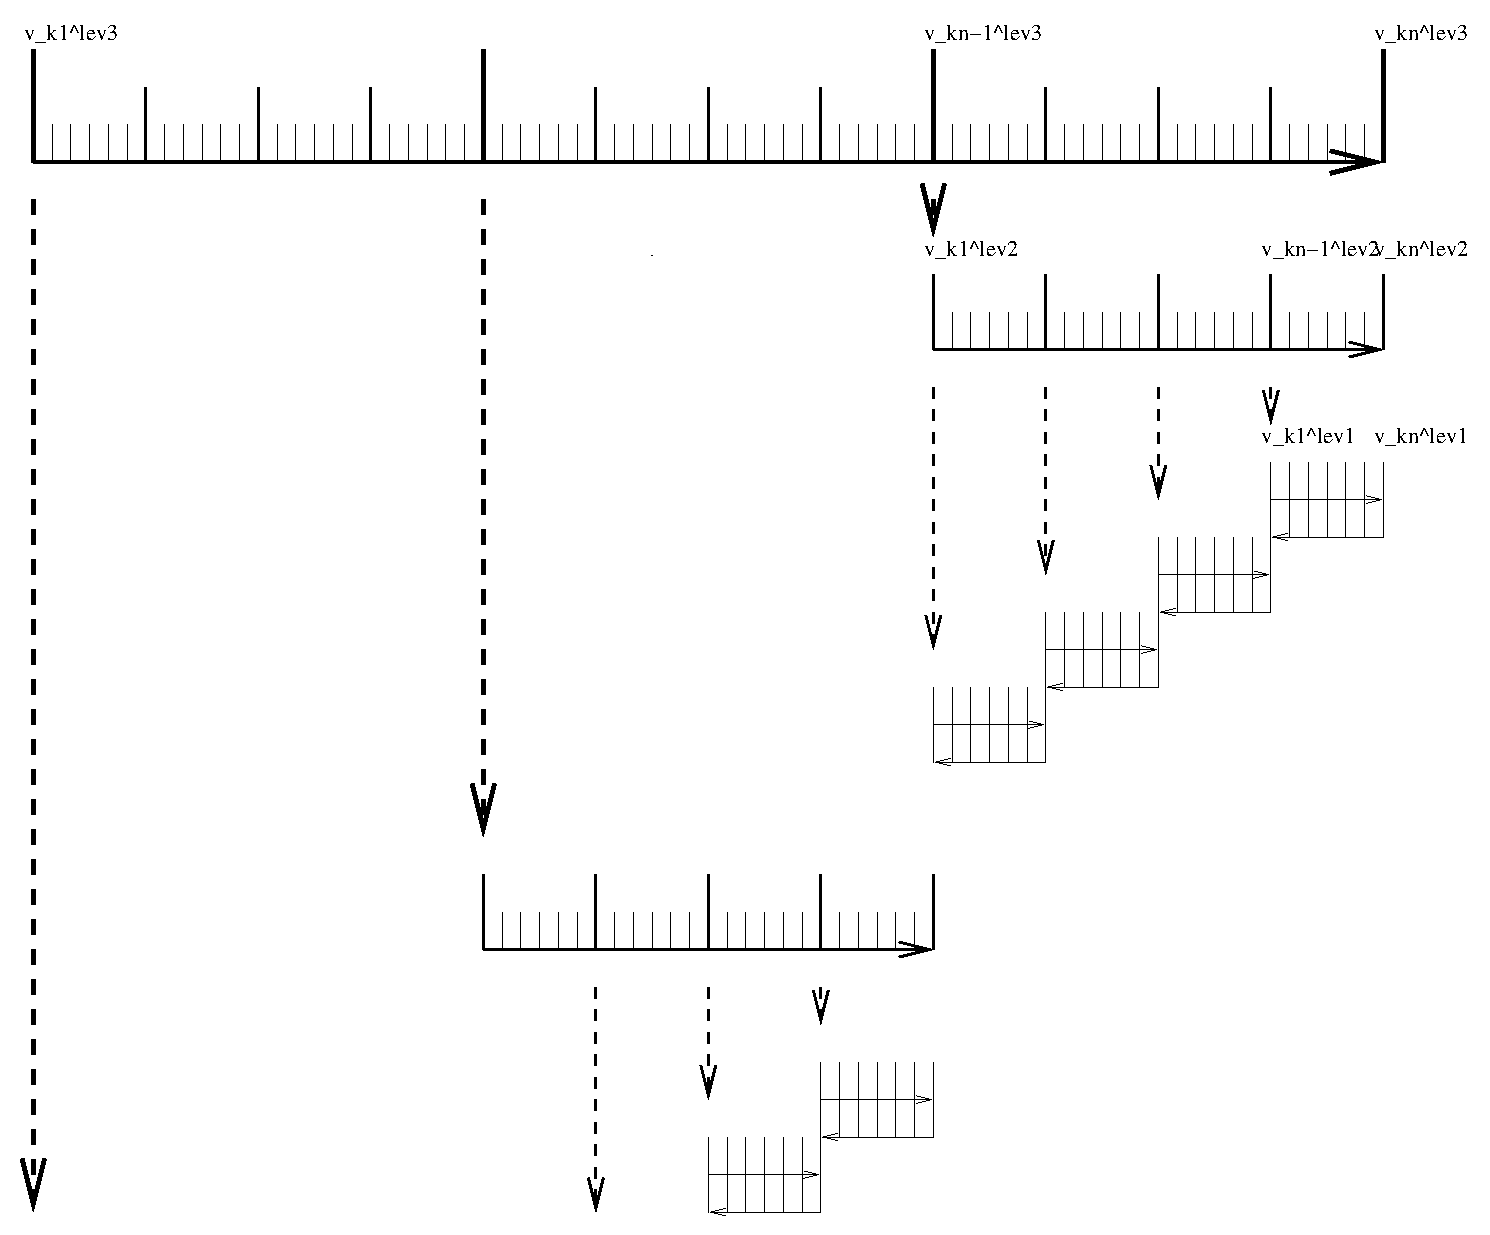
\epsfig{file=part5/checkpointing.eps, width=0.8\textwidth}}
%\psfull
\caption
{Schematic view of intermediate dump and restart for 
3-level checkpointing.}
\label{fig:3levelcheck}
\end{figure}

% \subsection{Optimal perturbations}
% \label{sec_optpert}


% \subsection{Error covariance estimate and Hessian matrix}
% \label{sec_hessian}

\newpage

%**********************************************************************
\section{AD-specific setup by example: sensitivity of carbon sequestration}
\label{sec_ad_setup_ex}
%**********************************************************************

The MITGCM has been adapted to enable AD using TAMC or TAF.
The present description, therefore, is specific to the
use of TAMC or TAF as AD tool.
The following sections describe the steps which are necessary to 
generate a tangent linear or adjoint model of the MITGCM.
We take as an example the sensitivity of carbon sequestration
in the ocean.
The AD-relevant hooks in the code are sketched in 
\reffig{adthemodel}, \reffig{adthemain}.

\subsection{Overview of the experiment}

We describe an adjoint sensitivity analysis of outgassing from 
the ocean into the atmosphere of a carbon-like tracer injected
into the ocean interior (see \cite{hil-eta:01}).

\subsubsection{Passive tracer equation}

For this work the MITGCM was augmented with a thermodynamically 
inactive tracer, $C$. Tracer residing in the ocean 
model surface layer is outgassed according to a relaxation time scale, 
$\mu$. Within the ocean interior, the tracer is passively advected 
by the ocean model currents. The full equation for the time evolution
%
\begin{equation}
\label{carbon_ddt}
\frac{\partial C}{\partial t} \, = \, 
-U\cdot \nabla C \, - \, \mu C \, + \, \Gamma(C) \,+ \, S
\end{equation}
%
also includes a source term $S$. This term 
represents interior sources of $C$ such as would arise due to
direct injection.
The velocity term, $U$, is the sum of the
model Eulerian circulation and an eddy-induced velocity, the latter
parameterized according to Gent/McWilliams 
(\cite{gen-mcw:90, gen-eta:95}).
The convection function, $\Gamma$, mixes $C$ vertically wherever the 
fluid is locally statically unstable. 

The outgassing time scale, $\mu$, in eqn. (\ref{carbon_ddt})
is set so that \( 1/\mu \sim 1 \ \mathrm{year} \) for the surface
ocean and $\mu=0$ elsewhere. With this value, eqn. (\ref{carbon_ddt})
is valid as a prognostic equation for small perturbations in oceanic 
carbon concentrations. This configuration provides a 
powerful tool for examining the impact of large-scale ocean circulation
on $ CO_2 $ outgassing due to interior injections.
As source we choose a constant in time injection of 
$ S = 1 \,\, {\rm mol / s}$.

\subsubsection{Model configuration}

The model configuration employed has a constant 
$4^\circ \times 4^\circ$ resolution horizontal grid and realistic 
geography and bathymetry. Twenty vertical layers are used with 
vertical spacing ranging
from 50 m near the surface to 815 m at depth. 
Driven to steady-state by climatalogical wind-stress, heat and
fresh-water forcing the model reproduces well known large-scale
features of the ocean general circulation. 

\subsubsection{Outgassing cost function}

To quantify and understand outgassing due to injections of $C$
in eqn. (\ref{carbon_ddt}),
we define a cost function $ {\cal J} $ that measures the total amount of 
tracer outgassed at each timestep:
%
\begin{equation}
\label{cost_tracer}
{\cal J}(t=T)=\int_{t=0}^{t=T}\int_{A} \mu C \, dA \, dt
\end{equation}
%
Equation(\ref{cost_tracer}) integrates the outgassing term, $\mu C$, 
from (\ref{carbon_ddt})
over the entire ocean surface area, $A$, and accumulates it 
up to time $T$.
Physically, ${\cal J}$ can be thought of as representing the amount of 
$CO_2$ that our model predicts would be outgassed following an
injection at rate $S$.
The sensitivity of ${\cal J}$ to the spatial location of $S$, 
$\frac{\partial {\cal J}}{\partial S}$,
can be used to identify regions from which circulation
would cause $CO_2$ to rapidly outgas following injection
and regions in which $CO_2$ injections would remain effectively 
sequesterd within the ocean.

\subsection{Code configuration}

The model configuration for this experiment resides under the
directory {\it verification/carbon/}.
The code customisation routines are in {\it verification/carbon/code/}:
%
\begin{itemize}
%
\item {\it .genmakerc}
%
\item {\it COST\_CPPOPTIONS.h}
%
\item {\it CPP\_EEOPTIONS.h}
%
\item {\it CPP\_OPTIONS.h}
%
\item {\it CTRL\_OPTIONS.h}
%
\item {\it ECCO\_OPTIONS.h}
%
\item {\it SIZE.h}
%
\item {\it adcommon.h}
%
\item {\it tamc.h}
%
\end{itemize}
%
The runtime flag and parameters settings are contained in 
{\it verification/carbon/input/},
together with the forcing fields and and restart files:
%
\begin{itemize}
%
\item {\it data}
%
\item {\it data.cost}
%
\item {\it data.ctrl}
%
\item {\it data.gmredi}
%
\item {\it data.grdchk}
%
\item {\it data.optim}
%
\item {\it data.pkg}
%
\item {\it eedata}
%
\item {\it topog.bin}
%
\item {\it windx.bin, windy.bin}
%
\item {\it salt.bin, theta.bin}
%
\item {\it SSS.bin, SST.bin}
%
\item {\it pickup*}
%
\end{itemize}
%
Finally, the file to generate the adjoint code resides in
$ adjoint/ $:
%
\begin{itemize}
%
\item {\it makefile}
%
\end{itemize}
%

Below we describe the customisations of this files which are
specific to this experiment.

\subsubsection{File {\it .genmakerc}}
This file overwrites default settings of {\it genmake}.
In the present example it is used to switch on the following
packages which are related to automatic differentiation
and are disabled by default: \\
\hspace*{4ex} {\tt set ENABLE=( autodiff cost ctrl ecco gmredi grdchk kpp )}  \\
Other packages which are not needed are switched off: \\
\hspace*{4ex} {\tt set DISABLE=( aim obcs zonal\_filt shap\_filt cal exf )}

\subsubsection{File {\it COST\_CPPOPTIONS.h,  CTRL\_OPTIONS.h}}

These files used to contain package-specific CPP-options
(see Section \ref{???}).
For technical reasons those options have been grouped together
in the file {\it ECCO\_OPTIONS.h}.
To retain the modularity, the files have been kept and contain
the standard include of the {\it CPP\_OPTIONS.h} file.

\subsubsection{File {\it CPP\_EEOPTIONS.h}}

This file contains 'wrapper'-specific CPP options.
It only needs to be changed if the code is to be run
in a parallel environment (see Section \ref{???}).

\subsubsection{File {\it CPP\_OPTIONS.h}}

This file contains model-specific CPP options
(see Section \ref{???}).
Most options are related to the forward model setup.
They are identical to the global steady circulation setup of
{\it verification/exp2/}.
The three options specific to this experiment are \\
\hspace*{4ex} {\tt \#define ALLOW\_PASSIVE\_TRACER} \\
This flag enables the code to carry through the
advection/diffusion of a passive tracer along the
model integration. \\
\hspace*{4ex} {\tt \#define ALLOW\_MIT\_ADJOINT\_RUN} \\
This flag enables the inclusion of some AD-related fields
concerning initialisation, link between control variables
and forward model variables, and the call to the top-level
forward/adjoint subroutine {\it adthe\_main\_loop}
instead of {\it the\_main\_loop}. \\
\hspace*{4ex} {\tt \#define ALLOW\_GRADIENT\_CHECK} \\
This flag enables the gradient check package.
After computing the unperturbed cost function and its gradient,
a series of computations are performed for which \\
$\bullet$ an element of the control vector is perturbed \\
$\bullet$ the cost function w.r.t. the perturbed element is
computed \\
$\bullet$ the difference between the perturbed and unperturbed
cost function is computed to compute the finite difference gradient \\
$\bullet$ the finite difference gradient is compared with the
adjoint-generated gradient.
The gradient check package is further described in Section ???.

\subsubsection{File {\it ECCO\_OPTIONS.h}}

The CPP options of several AD-related packages are grouped
in this file:
%
\begin{itemize}
%
\item 
Adjoint support package: {\it pkg/autodiff/} \\
This package contains hand-written adjoint code such as
active file handling, flow directives for files which must not
be differentiated, and TAMC-specific header files. \\
\hspace*{4ex} {\tt \#define ALLOW\_AUTODIFF\_TAMC} \\
defines TAMC-related features in the code. \\
\hspace*{4ex} {\tt \#define ALLOW\_TAMC\_CHECKPOINTING} \\
enables the checkpointing feature of TAMC
(see Section \ref{???}).
In the present example a 3-level checkpointing is implemented.
The code contains the relevant store directives, common block
and tape initialisations, storing key computation,
and loop index handling.
The checkpointing length at each level is defined in
file {\it tamc.h}, cf. below.
%
\item Cost function package: {\it pkg/cost/} \\
This package contains all relevant routines for
initialising, accumulating and finalizing the cost function
(see Section \ref{???}). \\
\hspace*{4ex} {\tt \#define ALLOW\_COST} \\
enables all general aspects of the cost function handling,
in particular the hooks in the foorward code for
initialising, accumulating and finalizing the cost function. \\
\hspace*{4ex} {\tt \#define ALLOW\_COST\_TRACER} \\
includes the call to the cost function for this
particular experiment, eqn. (\ref{cost_tracer}).
%
\item Control variable package: {\it pkg/ctrl/} \\
This package contains all relevant routines for
the handling of the control vector.
Each control variable can be enabled/disabled with its own flag: \\
\begin{tabular}{ll}
\hspace*{2ex} {\tt \#define ALLOW\_THETA0\_CONTROL} & 
initial temperature \\
\hspace*{2ex} {\tt \#define ALLOW\_SALT0\_CONTROL} & 
initial salinity \\
\hspace*{2ex} {\tt \#define ALLOW\_TR0\_CONTROL} & 
initial passive tracer concentration \\
\hspace*{2ex} {\tt \#define ALLOW\_TAUU0\_CONTROL} & 
zonal wind stress \\
\hspace*{2ex} {\tt \#define ALLOW\_TAUV0\_CONTROL} & 
meridional wind stress \\
\hspace*{2ex} {\tt \#define ALLOW\_SFLUX0\_CONTROL} & 
freshwater flux \\
\hspace*{2ex} {\tt \#define ALLOW\_HFLUX0\_CONTROL} & 
heat flux \\
\hspace*{2ex} {\tt \#define ALLOW\_DIFFKR\_CONTROL} & 
diapycnal diffusivity \\
\hspace*{2ex} {\tt \#undef ALLOW\_KAPPAGM\_CONTROL} & 
isopycnal diffusivity \\
\end{tabular}
%
\end{itemize}

\subsubsection{File {\it SIZE.h}}

The file contains the grid point dimensions of the forward
model. It is identical to the {\it verification/exp2/}: \\
\hspace*{4ex} {\tt sNx = 90} \\
\hspace*{4ex} {\tt sNy = 40} \\
\hspace*{4ex} {\tt Nr = 20} \\
It correpsponds to a single-tile/single-processor setup:
{\tt nSx = nSy = 1, nPx = nPy = 1},
with standard overlap dimensioning
{\tt OLx = OLy = 3}.

\subsubsection{File {\it adcommon.h}}

This file contains common blocks of some adjoint variables
that are generated by TAMC. 
The common blocks are used by the adjoint support routine
{\it addummy\_in\_stepping} which needs to access those variables:

\begin{tabular}{ll}
\hspace*{4ex} {\tt common /addynvars\_r/} &
\hspace*{4ex} is related to {\it DYNVARS.h} \\
\hspace*{4ex} {\tt common /addynvars\_cd/} &
\hspace*{4ex} is related to {\it DYNVARS.h} \\
\hspace*{4ex} {\tt common /addynvars\_diffkr/} &
\hspace*{4ex} is related to {\it DYNVARS.h} \\
\hspace*{4ex} {\tt common /addynvars\_kapgm/} &
\hspace*{4ex} is related to {\it DYNVARS.h} \\
\hspace*{4ex} {\tt common /adtr1\_r/} &
\hspace*{4ex} is related to {\it TR1.h} \\
\hspace*{4ex} {\tt common /adffields/} &
\hspace*{4ex} is related to {\it FFIELDS.h}\\
\end{tabular}

Note that if the structure of the common block changes in the 
above header files of the forward code, the structure
of the adjoint common blocks will change accordingly.
Thus, it has to be made sure that the structure of the
adjoint common block in the hand-written file {\it adcommon.h}
complies with the automatically generated adjoint common blocks
in {\it adjoint\_model.F}.

\subsubsection{File {\it tamc.h}}

This routine contains the dimensions for TAMC checkpointing.
%
\begin{itemize}
%
\item {\tt \#ifdef ALLOW\_TAMC\_CHECKPOINTING} \\
3-level checkpointing is enabled, i.e. the timestepping
is divided into three different levels (see Section \ref{???}).
The model state of the outermost ({\tt nchklev\_3}) and the
intermediate ({\tt nchklev\_2}) timestepping loop are stored to file
(handled in {\it the\_main\_loop}).
The innermost loop ({\tt nchklev\_1}) 
avoids I/O by storing all required variables
to common blocks. This storing may also be necessary if
no checkpointing is chosen
(nonlinear functions, if-statements, iterative loops, ...).
In the present example the dimensions are chosen as follows: \\
\hspace*{4ex} {\tt nchklev\_1      =  36 } \\
\hspace*{4ex} {\tt nchklev\_2      =  30 } \\
\hspace*{4ex} {\tt nchklev\_3      =  60 } \\
To guarantee that the checkpointing intervals span the entire
integration period the following relation must be satisfied: \\
\hspace*{4ex} {\tt nchklev\_1*nchklev\_2*nchklev\_3 $ \ge $ nTimeSteps} \\
where {\tt nTimeSteps} is either specified in {\it data}
or computed via \\
\hspace*{4ex} {\tt nTimeSteps = (endTime-startTime)/deltaTClock }. 
%
\item {\tt \#undef ALLOW\_TAMC\_CHECKPOINTING} \\
No checkpointing is enabled.
In this case the relevant counter is {\tt nchklev\_0}.
Similar to above, the following relation has to be satisfied \\
\hspace*{4ex} {\tt nchklev\_0 $ \ge $ nTimeSteps}.
%
\end{itemize}

The following parameters may be worth describing: \\
%
\hspace*{4ex} {\tt isbyte} \\
\hspace*{4ex} {\tt maxpass} \\
~
 
\subsubsection{File {\it makefile}}

This file contains all relevant paramter flags and
lists to run TAMC or TAF.
It is assumed that TAMC is available to you, either locally,
being installed on your network, or remotely through the 'TAMC Utility'.
TAMC is called with the command {\tt tamc} followed by a
number of options. They are described in detail in the
TAMC manual \cite{gie:99}.
Here we briefly discuss the main flags used in the {\it makefile}
%
\begin{itemize}
\item [{\tt tamc}] {\tt
-input <variable names>
-output <variable name> -r4 ... \\
-toplevel <S/R name> -reverse <file names> 
}
\end{itemize}
%
\begin{itemize}
%
\item {\tt -toplevel <S/R name>} \\
Name of the toplevel routine, with respect to which the
control flow analysis is performed.
%
\item {\tt -input <variable names>} \\
List of independent variables $ u $ with respect to which the
dependent variable $ J $ is differentiated.
%
\item {\tt -output <variable name>} \\
Dependent variable $ J $  which is to be differentiated.
%
\item {\tt -reverse <file names>} \\
Adjoint code is generated to compute the sensitivity of an
independent variable w.r.t.  many dependent variables.
In the discussion of Section ???
the generated adjoint top-level routine computes the product
of the transposed Jacobian matrix $ M^T $ times
the gradient vector $ \nabla_v J $.
\\
{\tt <file names>} refers to the list of files {\it .f} which are to be
analyzed by TAMC. This list is generally smaller than the full list
of code to be compiled. The files not contained are either
above the top-level routine (some initialisations), or are
deliberately hidden from TAMC, either because hand-written
adjoint routines exist, or the routines must not (or don't have to)
be differentiated. For each routine which is part of the flow tree
of the top-level routine, but deliberately hidden from TAMC
(or for each package which contains such routines),
a corresponding file {\it .flow} exists containing flow directives
for TAMC.
%
\item {\tt -r4} \\
~
%
\end{itemize}


\subsubsection{File {\it data}}

\subsubsection{File {\it data.cost}}

\subsubsection{File {\it data.ctrl}}

\subsubsection{File {\it data.gmredi}}

\subsubsection{File {\it data.grdchk}}

\subsubsection{File {\it data.optim}}

\subsubsection{File {\it data.pkg}}

\subsubsection{File {\it eedata}}

\subsubsection{File {\it topog.bin}}

\subsubsection{File {\it windx.bin, windy.bin}}

\subsubsection{File {\it salt.bin, theta.bin}}

\subsubsection{File {\it SSS.bin, SST.bin}}

\subsubsection{File {\it pickup*}}

\subsection{Compiling the model and its adjoint} 

\newpage 

%**********************************************************************
\section{TLM and ADM generation in general}
\label{sec_ad_setup_gen}
%**********************************************************************

In this section we describe in a general fashion 
the parts of the code that are relevant for automatic
differentiation using the software tool TAMC. 

\begin{figure}[b!]
% $Header: /u/gcmpack/manual/s_autodiff/text/doc_ad_the_model.tex,v 1.1.1.1 2001/08/08 16:16:26 adcroft Exp $
% $Name:  $

{\small
\begin{verbatim}
   **************
   the_model_main
   **************
   |
   |--- initialise_fixed
   |    |
   |   ...
   |    |--- packages_readparms
   |    |    |
   |    |   ...
   |    |    |--- #ifdef ALLOW_ADJOINT_RUN
   |    |    |           call cost_readparms
   |    |    |           call ctrl_readparms
   |    |    |    #endif
   |    |   ...
   |    |    o
   |   ...
   |    o
  ...
   |
   |--- #ifdef ALLOW_ADJOINT_RUN
   |           call ctrl_unpack
   |           call adthe_main_loop
   |           call ctrl_pack
   |    #else
   |           call the_main_loop
   |    #endif
   |
   |--- #ifdef ALLOW_GRADIENT_CHECK
   |           call grdchk_main
   |    #endif
  ...
   o
\end{verbatim}
}

\caption{~}
\label{fig:adthemodel}
\end{figure}

The basic flow is depicted in \reffig{adthemodel}.
If the option {\tt ALLOW\_AUTODIFF\_TAMC} is defined, the driver routine
{\it the\_model\_main}, instead of calling {\it the\_main\_loop},
invokes the adjoint of this routine, {\it adthe\_main\_loop},
which is the toplevel routine in terms of reverse mode computation.
The routine {\it adthe\_main\_loop} has been generated using TAMC.
It contains both the forward integration of the full model, 
any additional storing that is required for efficient checkpointing, 
and the reverse integration of the adjoint model.
The structure of {\it adthe\_main\_loop} has been strongly
simplified for clarification; in particular, no checkpointing
procedures are shown here.
Prior to the call of {\it adthe\_main\_loop}, the routine
{\it ctrl\_unpack} is invoked to unpack the control vector,
and following that call, the routine {\it ctrl\_pack}
is invoked to pack the control vector
(cf. Section \ref{section_ctrl}).
If gradient checks are to be performed, the option 
{\tt ALLOW\_GRADIENT\_CHECK} is defined. In this case
the driver routine {\it grdchk\_main} is called after
the gradient has been computed via the adjoint
(cf. Section \ref{section_grdchk}).

\subsection{The cost function (dependent variable)
\label{section_cost}}

The cost function $ {\cal J} $ is referred to as the {\sf dependent variable}.
It is a function of the input variables $ \vec{u} $ via the composition
$ {\cal J}(\vec{u}) \, = \, {\cal J}(M(\vec{u})) $. 
The input is referred to as the
{\sf independent variables} or {\sf control variables}.
All aspects relevant to the treatment of the cost function $ {\cal J} $
(parameter setting, initialisation, accumulation, 
final evaluation), are controlled by the package {\it pkg/cost}.

\begin{figure}[h!]
\begin{figure}[h!]

{\scriptsize
\begin{verbatim}
      the_model_main
      |
      |-- initialise_fixed
      |   |
      |   |-- packages_readparms
      |       |
      |       |-- cost_readparms
      |       o
      |
      |-- the_main_loop
     ...  |
          |-- initialise_varia
          |   |
          |   |-- packages_init_variables
          |       |
          |       |-- cost_init
          |       o
          |
          |-- do iloop = 1,nTimeSteps
          |      |-- forward_step
          |      |-- cost_tile
          |      |   |
          |      |   |-- cost_tracer
          |   end do
          |
          |-- cost_final
          o
\end{verbatim}
}

\caption{~}
\label{fig:costflow}
\end{figure}

\caption{~}
\label{fig:costflow}
\end{figure}

\subsubsection{genmake and CPP options}
%
\begin{itemize}
%
\item 
\fbox{
\begin{minipage}{12cm}
{\it genmake}, {\it CPP\_OPTIONS.h}, {\it ECCO\_CPPOPTIONS.h}
\end{minipage}
}
\end{itemize}
%
The directory {\it pkg/cost} can be included to the
compile list in 3 different ways (cf. Section \ref{???}):
%
\begin{enumerate}
%
\item {\it genmake}: \\
Change the default settings in the file {\it genmake} by adding 
{\bf cost} to the {\bf enable} list (not recommended).
%
\item {\it .genmakerc}: \\
Customize the settings of {\bf enable}, {\bf disable} which are
appropriate for your experiment in the file {\it .genmakerc} 
and add the file to your compile directory.
%
\item genmake-options: \\
Call {\it genmake} with the option
{\tt genmake -enable=cost}.
%
\end{enumerate}
The basic CPP option to enable the cost function is {\bf ALLOW\_COST}.
Each specific cost function contribution has its own option.
For the present example the option is {\bf ALLOW\_COST\_TRACER}.
All cost-specific options are set in {\it ECCO\_CPPOPTIONS.h}
Since the cost function is usually used in conjunction with
automatic differentiation, the CPP option
{\bf ALLOW\_ADJOINT\_RUN} should be defined
(file {\it CPP\_OPTIONS.h}).

\subsubsection{Initialisation}
%
The initialisation of the {\it cost} package is readily enabled
as soon as the CPP option {\bf ALLOW\_ADJOINT\_RUN} is defined.
%
\begin{itemize}
%
\item 
\fbox{
\begin{minipage}{12cm}
Parameters: {\it cost\_readparms}
\end{minipage}
}
\\
This S/R 
reads runtime flags and parameters from file {\it data.cost}.
For the present example the only relevant parameter read
is {\bf mult\_tracer}. This multiplier enables different
cost function contributions to be switched on
( = 1.) or off ( = 0.) at runtime.
For more complex cost functions which involve model vs. data
misfits, the corresponding data filenames and data
specifications (start date and time, period, ...) are read
in this S/R.
%
\item 
\fbox{
\begin{minipage}{12cm}
Variables: {\it cost\_init}
\end{minipage}
}
\\
This S/R 
initialises the different cost function contributions.
The contribtion for the present example is {\bf objf\_tracer}
which is defined on each tile (bi,bj).
%
\end{itemize}
%
\subsubsection{Accumulation}
%
\begin{itemize}
%
\item 
\fbox{
\begin{minipage}{12cm}
{\it cost\_tile}, {\it cost\_tracer}
\end{minipage}
}
\end{itemize}
%
The 'driver' routine
{\it cost\_tile} is called at the end of each time step.
Within this 'driver' routine, S/R are called for each of
the chosen cost function contributions.
In the present example ({\bf ALLOW\_COST\_TRACER}),
S/R {\it cost\_tracer} is called.
It accumulates {\bf objf\_tracer} according to eqn. (\ref{???}).
%
\subsubsection{Finalize all contributions}
%
\begin{itemize}
%
\item 
\fbox{
\begin{minipage}{12cm}
{\it cost\_final}
\end{minipage}
}
\end{itemize}
%
At the end of the forward integration S/R {\it cost\_final}
is called. It accumulates the total cost function {\bf fc}
from each contribution and sums over all tiles:
\begin{equation}
{\cal J} \, = \, 
{\rm fc} \, = \, 
{\rm mult\_tracer} \sum_{bi,\,bj}^{nSx,\,nSy}
{\rm objf\_tracer}(bi,bj) \, + \, ...
\end{equation}
%
The total cost function {\bf fc} will be the
'dependent' variable in the argument list for TAMC, i.e.
\begin{verbatim}
tamc -output 'fc' ...
\end{verbatim}

%%%% \end{document}

\begin{figure}
% $Header: /u/gcmpack/manual/s_autodiff/text/doc_ad_the_main.tex,v 1.1.1.1 2001/08/08 16:16:26 adcroft Exp $
% $Name:  $

{\small
\begin{verbatim}
   *************
   the_main_loop
   *************
   |
   |--- initialise_varia
   |    |
   |   ...
   |    |--- packages_init_varia
   |    |    |
   |    |   ...
   |    |    |--- #ifdef ALLOW_ADJOINT_RUN
   |    |    |          call ctrl_map_ini
   |    |    |          call cost_ini
   |    |    |    #endif
   |    |   ...
   |    |    o
   |   ...
   |    o
  ...
   |--- #ifdef ALLOW_ADJOINT_RUN
   |          call ctrl_map_forcing
   |    #endif
  ...
   |--- #ifdef ALLOW_TAMC_CHECKPOINTING
              do ilev_3 = 1,nchklev_3
   |            do ilev_2 = 1,nchklev_2
   |              do ilev_1 = 1,nchklev_1
   |                iloop = (ilev_3-1)*nchklev_2*nchklev_1 +
   |                        (ilev_2-1)*nchklev_1           + ilev_1
   |    #else
   |          do iloop = 1, nTimeSteps
   |    #endif
   |    |
   |    |---       call forward_step
   |    |
   |    |--- #ifdef ALLOW_COST
   |    |          call cost_tile
   |    |    #endif
   |    |
   |    |    enddo
   |    o
   |
   |--- #ifdef ALLOW_COST
   |          call cost_final
   |    #endif
   o
\end{verbatim}
}

\caption{~}
\label{fig:adthemain}
\end{figure}

\subsection{The control variables (independent variables)
\label{section_ctrl}}

The control variables are a subset of the model input
(initial conditions, boundary conditions, model parameters).
Here we identify them with the variable $ \vec{u} $.
All intermediate variables whose derivative w.r.t. control
variables do not vanish are called {\sf active variables}.
All subroutines whose derivative w.r.t. the control variables
don't vanish are called {\sf active routines}.
Read and write operations from and to file can be viewed
as variable assignments. Therefore, files to which
active variables are written and from which active variables
are read are called {\sf active files}.
All aspects relevant to the treatment of the control variables
(parameter setting, initialisation, perturbation)
are controled by the package {\it pkg/ctrl}.

\begin{figure}[h!]
\begin{figure}[!ht]

{\scriptsize
\begin{verbatim}
          the_model_main
          |
          |-- initialise_fixed
          |   |
          |   |-- packages_readparms
          |       |
          |       |-- ctrl_init                - initialise control
          |       o                              package
          |
          |-- ctrl_unpack                      - unpack control vector
          |
          |-- adthe_main_loop                  - forward/adjoint run
          |   |
          |   |-- initialise_variables
          |   |   |
          |   |   |-- packages_init_variables
          |   |       |
          |   |       |-- ctrl_map_ini         - link init. state and
          |   |       o                          parameters to control 
          |   |                                  variables
          |   |-- ctrl_map_forcing             - link forcing fields to
          |  ...                                 control variables
          |
          |-- ctrl_pack                        - pack control vector
\end{verbatim}
}
\caption{~}
\label{fig:ctrlflow}
\end{figure}

\caption{~}
\label{fig:ctrlflow}
\end{figure}

\subsubsection{genmake and CPP options}
%
\begin{itemize}
%
\item 
\fbox{
\begin{minipage}{12cm}
{\it genmake}, {\it CPP\_OPTIONS.h}, {\it ECCO\_CPPOPTIONS.h}
\end{minipage}
}
\end{itemize}
%
To enable the directory to be included to the compile list,
{\bf ctrl} has to be added to the {\bf enable} list in
{\it .genmakerc} (or {\it genmake} itself).
Each control variable is enabled via its own CPP option
in {\it ECCO\_CPPOPTIONS.h}.

\subsubsection{Initialisation}
%
\begin{itemize}
%
\item 
\fbox{
\begin{minipage}{12cm}
Parameters: {\it ctrl\_readparms}
\end{minipage}
}
\\
%
This S/R 
reads runtime flags and parameters from file {\it data.ctrl}.
For the present example the file contains the file names
of each control variable that is used.
In addition, the number of wet points for each control
variable and the net dimension of the space of control
variables (counting wet points only) {\bf nvarlength}
is determined.
Masks for wet points for each tile {\bf (bi,\,bj)}
and vertical layer {\bf k} are generated for the three
relevant categories on the C-grid:
{\bf nWetCtile} for tracer fields, 
{\bf nWetWtile} for zonal velocity fields,
{\bf nWetStile} for meridional velocity fields.
%
\item 
\fbox{
\begin{minipage}{12cm}
Control variables, control vector,
and their gradients: {\it ctrl\_unpack}
\end{minipage}
}
\\
%
Two important issues related to the handling of the control
variables in the MITGCM need to be addressed.
First, in order to save memory, the control variable arrays
are not kept in memory, but rather read from file and added
to the initial fields during the model initialisation phase.
Similarly, the corresponding adjoint fields which represent
the gradient of the cost function w.r.t. the control variables
are written to file at the end of the adjoint integration.
Second, in addition to the files holding the 2-dim. and 3-dim.
control variables and the corresponding cost gradients, 
a 1-dim. {\sf control vector} 
and {\sf gradient vector} are written to file. They contain 
only the wet points of the control variables and the corresponding 
gradient.
This leads to a significant data compression.
Furthermore, an option is available
({\tt ALLOW\_NONDIMENSIONAL\_CONTROL\_IO}) to
non-dimensionalise the control and gradient vector,
which otherwise would contain different pieces of different
magnitudes and units.
Finally, the control and gradient vector can be passed to a 
minimization routine if an update of the control variables
is sought as part of a minimization exercise.

The files holding fields and vectors of the control variables
and gradient are generated and initialised in S/R {\it ctrl\_unpack}.
%
\end{itemize}

\subsubsection{Perturbation of the independent variables}
%
The dependency flow for differentiation w.r.t. the controls 
starts with adding a perturbation onto the input variable,
thus defining the independent or control variables for TAMC.
Three types of controls may be considered:
%
\begin{itemize}
%
\item 
\fbox{
\begin{minipage}{12cm}
{\it ctrl\_map\_ini} (initial value sensitivity): 
\end{minipage}
}
\\
%
Consider as an example the initial tracer distribution
{\bf tr1} as control variable.
After {\bf tr1} has been initialised in
{\it ini\_tr1} (dynamical variables such as
temperature and salinity are initialised in {\it ini\_fields}),
a perturbation anomaly is added to the field in S/R
{\it ctrl\_map\_ini}
%
\begin{equation}
\begin{split}
u         & = \, u_{[0]} \, + \, \Delta u \\
{\bf tr1}(...) & = \, {\bf tr1_{ini}}(...) \, + \, {\bf xx\_tr1}(...)
\label{perturb}
\end{split}
\end{equation}
%
{\bf xx\_tr1} is a 3-dim. global array 
holding the perturbation. In the case of a simple
sensitivity study this array is identical to zero.
However, it's specification is essential in the context
of automatic differentiation since TAMC
treats the corresponding line in the code symbolically
when determining the differentiation chain and its origin.
Thus, the variable names are part of the argument list
when calling TAMC: 
%
\begin{verbatim}
tamc -input 'xx_tr1 ...' ...
\end{verbatim}
%
Now, as mentioned above, the MITGCM avoids maintaining
an array for each control variable by reading the
perturbation to a temporary array from file.
To ensure the symbolic link to be recognized by TAMC, a scalar
dummy variable {\bf xx\_tr1\_dummy} is introduced
and an 'active read' routine of the adjoint support
package {\it pkg/autodiff} is invoked.
The read-procedure is tagged with the variable
{\bf xx\_tr1\_dummy} enabbling TAMC to recognize the
initialisation of the perturbation.
The modified call of TAMC thus reads
%
\begin{verbatim}
tamc -input 'xx_tr1_dummy ...' ...
\end{verbatim}
%
and the modified operation to (\ref{perturb})
in the code takes on the form
%
\begin{verbatim}
       call active_read_xyz( 
     &      ..., tmpfld3d, ..., xx_tr1_dummy, ... )

       tr1(...) = tr1(...) + tmpfld3d(...)
\end{verbatim}
%
Note, that reading an active variable corresponds
to a variable assignment. Its derivative corresponds
to a write statement of the adjoint variable.
The 'active file' routines have been designed
to support active read and corresponding adjoint active write
operations (and vice versa).
%
\item 
\fbox{
\begin{minipage}{12cm}
{\it ctrl\_map\_forcing} (boundary value sensitivity): 
\end{minipage}
}
\\
%
The handling of boundary values as control variables
proceeds exactly analogous to the initial values
with the symbolic perturbation taking place in S/R
{\it ctrl\_map\_forcing}.
Note however an important difference:
Since the boundary values are time dependent with a new
forcing field applied at each time steps,
the general problem may be thought of as
a new control variable at each time step
(or, if the perturbation is averaged over a certain period,
at each $ N $ timesteps), i.e.
\[
u_{\rm forcing} \, = \,
\{ \, u_{\rm forcing} ( t_n ) \, \}_{
n \, = \, 1, \ldots , {\rm nTimeSteps} }
\]
%
In the current example an equilibrium state is considered,
and only an initial perturbation to
surface forcing is applied with respect to the
equilibrium state.
A time dependent treatment of the surface forcing is 
implemented in the ECCO environment, involving the
calendar ({\it cal}~) and external forcing ({\it exf}~) packages.
%
\item 
\fbox{
\begin{minipage}{12cm}
{\it ctrl\_map\_params} (parameter sensitivity): 
\end{minipage}
}
\\
%
This routine is not yet implemented, but would proceed
proceed along the same lines as the initial value sensitivity.
The mixing parameters {\bf diffkr} and {\bf kapgm}
are currently added as controls in {\it ctrl\_map\_ini.F}.
%
\end{itemize}
%

\subsubsection{Output of adjoint variables and gradient}
%
Several ways exist to generate output of adjoint fields.
%
\begin{itemize}
%
\item 
\fbox{
\begin{minipage}{12cm}
{\it ctrl\_map\_ini, ctrl\_map\_forcing}: 
\end{minipage}
}
\\
\begin{itemize}
%
\item {\bf xx\_...}: the control variable fields \\
Before the forward integration, the control
variables are read from file {\bf xx\_ ...} and added to
the model field.
%
\item {\bf adxx\_...}: the adjoint variable fields, i.e. the gradient
$ \nabla _{u}{\cal J} $ for each control variable \\
After the adjoint integration the corresponding adjoint
variables are written to {\bf adxx\_ ...}.
%
\end{itemize}
%
\item 
\fbox{
\begin{minipage}{12cm}
{\it ctrl\_unpack, ctrl\_pack}: 
\end{minipage}
}
\\
%
\begin{itemize}
%
\item {\bf vector\_ctrl}: the control vector \\
At the very beginning of the model initialisation,
the updated compressed control vector is read (or initialised)
and distributed to 2-dim. and 3-dim. control variable fields.
%
\item {\bf vector\_grad}: the gradient vector \\
At the very end of the adjoint integration,
the 2-dim. and 3-dim. adjoint variables are read,
compressed to a single vector and written to file.
%
\end{itemize}
%
\item 
\fbox{
\begin{minipage}{12cm}
{\it addummy\_in\_stepping}: 
\end{minipage}
}
\\
In addition to writing the gradient at the end of the
forward/adjoint integration, many more adjoint variables
of the model state
at intermediate times can be written using S/R 
{\it addummy\_in\_stepping}.
This routine is part of the adjoint support package 
{\it pkg/autodiff} (cf.f. below).
To be part of the adjoint code, the corresponding S/R
{\it dummy\_in\_stepping} has to be called in the forward
model (S/R {\it the\_main\_loop}) at the appropriate place.

{\it dummy\_in\_stepping} is essentially empty,
the corresponding adjoint routine is hand-written rather
than generated automatically.
Appropriate flow directives ({\it dummy\_in\_stepping.flow})
ensure that TAMC does not automatically 
generate {\it addummy\_in\_stepping} by trying to differentiate
{\it dummy\_in\_stepping}, but instead refers to 
the hand-written routine.

{\it dummy\_in\_stepping} is called in the forward code
at the beginning of each
timestep, before the call to {\it dynamics}, thus ensuring
that {\it addummy\_in\_stepping} is called at the end of
each timestep in the adjoint calculation, after the call to
{\it addynamics}.

{\it addummy\_in\_stepping} includes the header files
{\it adcommon.h}.
This header file is also hand-written. It contains
the common blocks 
{\bf /addynvars\_r/}, {\bf /addynvars\_cd/},
{\bf /addynvars\_diffkr/}, {\bf /addynvars\_kapgm/},
{\bf /adtr1\_r/}, {\bf /adffields/},
which have been extracted from the adjoint code to enable
access to the adjoint variables.
%
\end{itemize}


\subsubsection{Control variable handling for 
optimization applications}

In optimization mode the cost function $ {\cal J}(u) $ is sought
to be minimized with respect to a set of control variables
$ \delta {\cal J} \, = \, 0 $, in an iterative manner.
The gradient $ \nabla _{u}{\cal J} |_{u_{[k]}} $ together
with the value of the cost function itself $ {\cal J}(u_{[k]}) $ 
at iteration step $ k $ serve
as input to a minimization routine (e.g. quasi-Newton method,
conjugate gradient, ... \cite{gil_lem:89}) 
to compute an update in the
control variable for iteration step $k+1$
\[
u_{[k+1]} \, = \,  u_{[0]} \, + \, \Delta u_{[k+1]}
\quad \mbox{satisfying} \quad
 {\cal J} \left( u_{[k+1]} \right) \, < \, {\cal J} \left( u_{[k]} \right)
\]
$ u_{[k+1]} $ then serves as input for a forward/adjoint run
to determine $ {\cal J} $ and $ \nabla _{u}{\cal J} $ at iteration step
$ k+1 $.
Tab. \ref{???} sketches the flow between forward/adjoint model
and the minimization routine.

\begin{eqnarray*}
\scriptsize
\begin{array}{ccccc}
u_{[0]} \,\, ,  \,\, \Delta u_{[k]}    & ~ & ~ & ~ & ~ \\
{\Big\downarrow} 
   & ~ & ~ & ~ & ~ \\
 ~ & ~ & ~ & ~ & ~ \\
\hline
\multicolumn{1}{|c}{~} & ~ & ~ & ~ & \multicolumn{1}{c|}{~} \\
\multicolumn{1}{|c}{
u_{[k]} = u_{[0]} + \Delta u_{[k]}} &
\stackrel{\bf forward}{\bf \longrightarrow} &
v_{[k]} = M \left( u_{[k]} \right) &
\stackrel{\bf forward}{\bf \longrightarrow} &
\multicolumn{1}{c|}{
{\cal J}_{[k]} = {\cal J} \left( M \left( u_{[k]} \right) \right)} \\
\multicolumn{1}{|c}{~} & ~ & ~ & ~ & \multicolumn{1}{c|}{~} \\
\hline
\multicolumn{1}{|c}{~} & ~ & ~ & ~ & \multicolumn{1}{c|}{~}  \\
\multicolumn{1}{|c}{~} & ~ & ~ & ~ & \multicolumn{1}{c|}{{\Big\downarrow}} \\
\multicolumn{1}{|c}{~} & ~ & ~ & ~ & \multicolumn{1}{c|}{~}  \\
\hline
\multicolumn{1}{|c}{~} & ~ & ~ & ~ & \multicolumn{1}{c|}{~} \\
\multicolumn{1}{|c}{
\nabla_u {\cal J}_{[k]} (\delta {\cal J}) = 
T^{\ast} \cdot \nabla_v {\cal J} |_{v_{[k]}} (\delta {\cal J})} &
\stackrel{\bf adjoint}{\mathbf \longleftarrow} &
ad \, v_{[k]} (\delta {\cal J}) = 
\nabla_v {\cal J} |_{v_{[k]}} (\delta {\cal J}) &
\stackrel{\bf adjoint}{\mathbf \longleftarrow} &
\multicolumn{1}{c|}{ ad \, {\cal J} = \delta {\cal J}} \\
\multicolumn{1}{|c}{~} & ~ & ~ & ~ & \multicolumn{1}{c|}{~} \\
\hline
 ~ & ~ & ~ & ~ & ~ \\
\hspace*{15ex}{\Bigg\downarrow}  
\quad {\cal J}_{[k]}, \quad \nabla_u {\cal J}_{[k]}
 & ~ & ~ & ~ & ~ \\
 ~ & ~ & ~ & ~ & ~ \\
\hline
\multicolumn{1}{|c}{~} & ~ & ~ & ~ & \multicolumn{1}{c|}{~} \\
\multicolumn{1}{|c}{
{\cal J}_{[k]} \,\, ,  \,\, \nabla_u {\cal J}_{[k]}} &
{\mathbf \longrightarrow} & \text{\bf minimisation} &
{\mathbf \longrightarrow} & 
\multicolumn{1}{c|}{ \Delta u_{[k+1]}} \\
\multicolumn{1}{|c}{~} & ~ & ~ & ~ & \multicolumn{1}{c|}{~} \\
\hline
 ~ & ~ & ~ & ~ & ~ \\
 ~ & ~ & ~ & ~ & \Big\downarrow \\
 ~ & ~ & ~ & ~ & \Delta u_{[k+1]} \\
\end{array}
\end{eqnarray*}

The routines {\it ctrl\_unpack} and {\it ctrl\_pack} provide
the link between the model and the minimization routine.
As described in Section \ref{???} 
the {\it unpack} and {\it pack} routines read and write
control and gradient {\it vectors} which are compressed
to contain only wet points, in addition to the full
2-dim. and 3-dim. fields. 
The corresponding I/O flow looks as follows:

\vspace*{0.5cm}

{\scriptsize
\begin{tabular}{ccccc}
{\bf vector\_ctrl\_$<$k$>$ } & ~ & ~ & ~ & ~ \\
{\big\downarrow}  & ~ & ~ & ~ & ~ \\
\cline{1-1}
\multicolumn{1}{|c|}{\it ctrl\_unpack} & ~ & ~ & ~ & ~ \\
\cline{1-1}
{\big\downarrow}  & ~ & ~ & ~ & ~ \\
\cline{3-3}
\multicolumn{1}{l}{\bf xx\_theta0...$<$k$>$} & ~ &
\multicolumn{1}{|c|}{~} & ~ & ~ \\
\multicolumn{1}{l}{\bf xx\_salt0...$<$k$>$} & 
$\stackrel{\mbox{read}}{\longrightarrow}$ &
\multicolumn{1}{|c|}{forward integration} & ~ & ~ \\ 
\multicolumn{1}{l}{\bf \vdots} & ~ & \multicolumn{1}{|c|}{~}  
& ~ & ~ \\
\cline{3-3}
~ & ~ & $\downarrow$ & ~ & ~ \\
\cline{3-3}
~ & ~ & 
\multicolumn{1}{|c|}{~} & ~ & 
\multicolumn{1}{l}{\bf adxx\_theta0...$<$k$>$}  \\
~ & ~ & \multicolumn{1}{|c|}{adjoint integration} & 
$\stackrel{\mbox{write}}{\longrightarrow}$ & 
\multicolumn{1}{l}{\bf adxx\_salt0...$<$k$>$} \\ 
~ & ~ & \multicolumn{1}{|c|}{~}  
& ~ & \multicolumn{1}{l}{\bf \vdots} \\
\cline{3-3}
~ & ~ & ~ & ~ & {\big\downarrow} \\
\cline{5-5}
~ & ~ & ~ & ~ & \multicolumn{1}{|c|}{\it ctrl\_pack} \\
\cline{5-5}
~ & ~ & ~ & ~ &  {\big\downarrow} \\
~ & ~ & ~ & ~ &  {\bf vector\_grad\_$<$k$>$ } \\
\end{tabular}
}

\vspace*{0.5cm}


{\it ctrl\_unpack} reads the updated control vector
{\bf vector\_ctrl\_$<$k$>$}.
It distributes the different control variables to
2-dim. and 3-dim. files {\it xx\_...$<$k$>$}.
At the start of the forward integration the control variables
are read from {\it xx\_...$<$k$>$} and added to the
field.
Correspondingly, at the end of the adjoint integration
the adjoint fields are written
to {\it adxx\_...$<$k$>$}, again via the active file routines.
Finally, {\it ctrl\_pack} collects all adjoint files
and writes them to the compressed vector file
{\bf vector\_grad\_$<$k$>$}.

\subsection{TLM and ADM generation via TAMC}



\subsection{Flow directives and adjoint support routines \label{section_flowdir}}

\subsection{Store directives and checkpointing \label{section_checkpointing}}

\subsection{Gradient checks \label{section_grdchk}}

\subsection{Second derivative generation via TAMC}

\section{Example of adjoint code}
